\documentclass{report}
\usepackage{fullpage}
\usepackage{stmaryrd}
\usepackage{hyperref}
\usepackage{mathtools}
% \usepackage[english]{babel}
\usepackage{enumerate}  % enumarate styles
\usepackage{url}
\usepackage[pdftex]{graphicx}
\usepackage{amsmath}
\usepackage{amsfonts}
\usepackage{galois}
\usepackage{mathabx}
\usepackage{todonotes}
\usepackage{paralist}
\usepackage{multirow}
\usepackage{caption}
\usepackage{subfigure}
\usepackage{algorithmicx}
\usepackage[noend]{algpseudocode}
\usepackage{algorithm}
\usepackage{fancyvrb}
\usepackage{lscape}
\usepackage{listings}
\usepackage{pdflscape}
\usepackage{wrapfig}
\usepackage{etoolbox}
\usepackage{tikz}
\usetikzlibrary{shapes}
\usetikzlibrary{arrows}
\usetikzlibrary{positioning}
\usetikzlibrary{automata}
\usetikzlibrary{calc}

\lstset{
  basicstyle=\ttfamily,
  mathescape
}

% \lstset{
%   language=C
% }

\sloppy
% comment the following line to bring back the margins
\IfFileExists{./tmp/rm-margin.tex}{\input{tmp/rm-margin}}{}
% \usepackage[paperheight=19.5cm,paperwidth=12.4cm,margin=.1cm]{geometry}

% \usepackage{algorithm2e}

\makeatletter
\newcommand{\dashedrightarrow}[1][2pt]{%
  \settowidth{\@tempdima}{$\rightarrow$}\rightarrow% typeset arrow
  \makebox[-\@tempdima]{\hskip-1.5ex\color{white}\rule[0.5ex]{#1}{1pt}}% typeset overlay
  \phantom{\rightarrow}% advance appropriate horizontal distance
}
\makeatother

\newcommand{\ashu}[1]{ {\textcolor{magenta} {Ashutosh: #1}} }
\newcommand{\supratik}[1]{ {\textcolor{red} {Supratik: #1}} }
\newcommand{\divesh}[1]{ {\textcolor{blue} {Divyesh: #1}} }

\newcommand{\naturals}{\mathbb{N}}
\newcommand{\integers}{\mathbb{Z}}
\newcommand{\ordinals}{\mathbb{O}}
\newcommand{\numarals}{\mathbb{I}}

\newtheorem{df}{Definition}
\newcommand{\program}{P}
\newcommand{\sassign}{\;\mathtt{:=}\;}
\newcommand{\defeq}{\triangleq}
\newcommand{\assume}{\mathtt{assume}}
\newcommand{\formulas}{\Sigma}
\newcommand{\terms}{\mathcal{T}}

\newcommand{\ltrue}{\mathbf{tt}}
\newcommand{\lfalse}{\mathbf{ff}}
\newcommand{\limplies}{\Rightarrow}
\newcommand{\lxor}{\oplus}
\newcommand{\Land}{\bigwedge}
\newcommand{\Lor}{\bigvee}
\newcommand{\Lxor}{\bigoplus}
\newcommand{\lequiv}{\Leftrightarrow}
\newcommand{\landplus}{\mathrel{:\hspace{-3pt}\land\hspace{-3pt}=}}
\newcommand{\lorplus}{\mathrel{:\hspace{-3pt}\lor\hspace{-3pt}=}}

\newcommand{\maps}{\rightarrow}

\newcommand{\union}{{\cup} }
\newcommand{\Union}{{\bigcup} }
\newcommand{\powerset}{\mathcal{P}}
\newcommand{\intersection}{{\cap} }
\newcommand{\Intersection}{{\bigcap} }
\newcommand{\compose}{{\circ} }

\newcommand{\locationOf}[1]{loc(#1)}

\newcommand{\formula}{\phi}
\newcommand{\preds}{\pi}
\newcommand{\domain}{\mathcal{D}}

\newcommand{\smem}{\mathcal{S}}
\newcommand{\tout}{TO}


%algorithm names
\newcommand{\concolic}{concolic}

\newcommand{\correct}{\textsc{CORRECT}}

%tool names
% \newcommand{\ourtool}{$\crest^{+}$}
\newcommand{\ourtool}{\textsc{Crabs}}
\newcommand{\zthree}{\textsc{Z3}}
\newcommand{\crest}{\textsc{Crest}}
\newcommand{\synergy}{\textsc{Synergy}}
\newcommand{\cpachecker}{\textsc{CpaChecker}}
\newcommand{\fshell}{\textsc{Fshell}}
\newcommand{\svcomp}{\textsc{SvComp}}
\newcommand{\tiger}{\textsc{CpaTiger}}
\newcommand{\tara}{\textsc{Tara}}
\newcommand{\doublemp}{\mathtt{double\text{-}mp}}

\newcommand{\musketeer}{\textsc{Musketeer}}
\newcommand{\fender}{\textsc{Fender}}
\newcommand{\blender}{\textsc{Blender}}
\newcommand{\dfence}{\textsc{Dfence}}
\newcommand{\remmex}{\textsc{Remmex}}
\newcommand{\memorax}{\textsc{Memorax}}
\newcommand{\pensieve}{\textsc{Pensieve}}
\newcommand{\trencher}{\textsc{Trencher}}
\newcommand{\persist}{\textsc{Persist}}
\newcommand{\glue}{\textsc{Glue}}

\newcommand{\intel}{\textsc{Intel}}
\newcommand{\arm}{\textsc{ARM}}
\newcommand{\sparc}{\textsc{Sparc}}

\newtheorem{thm}{Theorem}

\newcommand{\rndbr}{RndBr}
\newcommand{\unfrnd}{UnfRnd}

%--------------------- DO NOT ERASE BELOW THIS LINE --------------------------

%%% Local Variables: 
%%% mode: latex
%%% TeX-master: "main"
%%% End: 


\setcounter{tocdepth}{10}
\setcounter{secnumdepth}{10}

\pagestyle{plain}

\begin{document}

\title{Matching Multiplications in Bit-Vector formulas\footnote{to appear in Proc. of International Conference on Verification, Model Checking and Abstract Interpretation (VMCAI), January 2017}}


%Names are in alphabetical order
%\author{Rahul Jain}
%\institute{School of Technology and Computer Science, Tata Institute of Fundamental Research}
%Supratik Chakraborty$^1$ \and Ashutosh Gupta$^2$ acknowledge 

%\date{\today}

\author{Rahul Jain}
\affil{School of Technology and Computer Science \\Tata Institute of Fundamental Research \\Mumbai}

\date{Dated: \today}

\maketitle

\begin{abstract}
%
%SMT solvers for the theory of fixed-width bit-vectors are widely used.
%
Bit-vector formulas arising from hardware verification problems often
contain word-level arithmetic operations.  Empirical evidence shows
that state-of-the-art SMT solvers are not very efficient at reasoning about
bit-vector formulas with multiplication.  This is particularly true
when multiplication operators are decomposed and represented in
alternative ways in the formula. %% In such cases, the solver may fail
%to identify the word-level
%% multiplication operation and end up bit-blasting..
%% %
%Therefore, it is important for an SMT solver to uses all the structure
%available in the problem, including the word-level reasoning.
%
%
We present a pre-processing heuristic that identifies certain types of
decomposed multipliers, and adds special assertions to the input
formula encoding the equivalence of sub-terms to word-level
multiplication.  The pre-processed formulas are then solved using an
SMT solver.  Our experiments with three  SMT solvers
show that our heuristic allows several formulas to be solved quickly,
while the same formulas time out without the pre-processing step.
%

%--------------------- DO NOT ERASE BELOW THIS LINE --------------------------

%%% Local Variables: 
%%% mode: latex
%%% TeX-master: "main"
%%% End: 

\end{abstract}


\centerline{\bfseries Acknowledgements}
\vspace{0.2 cm}

I would like to thank

\clearpage
\tableofcontents

%
\chapter{Introduction}
\label{sec:intro}
% Bit-vector is important
%
In recent years, SMT solving has emerged as a powerful technique for
testing, analysis and verification of hardware and software systems.
A wide variety of tools today use SMT solvers as part of their core
reasoning
engines~\cite{hwcbmc,boolector,ebmc,cbmc,corral,boogie,crv1,crv2,dart,concolic}.
%; examples include bounded model
%checkers~\cite{hwcbmc,boolector,ebmc,cbmc}, static assertion
%checkers~\cite{corral,boogie}, word-level symbolic trajectory
%evaluators~\cite{wste}, constrained test
%generators~\cite{crv1,crv2,dart}, concolic simulators~\cite{concolic},
%among others.
A common approach used in several of these tools is to model the
behaviour of a system using formulas in a combination of first-order
theories, and reduce the given problem to checking the
(un)satisfiability of a formula in the combined theory.  SMT solvers
play a central role in this approach, since they combine decision
procedures of individual first-order theories to check the
satisfiability of a formula in the combined theory.  Not surprisingly,
techniques to improve the performance of SMT solvers have attracted
significant attention over the years %% .  The literature contains a
%rich
%% body of heuristic strategies for improving the performance of
%% theory-specific solvers
(see~\cite{barrett,deMoura2013} for excellent expositions).  In this
paper, we add to the repertoire of such heuristics by proposing a
pre-processing step that analyzes an input formula, and adds specially
constructed assertions to it, without changing the semantics. We focus
on formulas in the quantifier-free theory of fixed-width bit-vectors
with multiplication, and show by means of experiments that three
state-of-the-art SMT solvers benefit significantly from our heuristic
when solving many benchmarks with multiplication operators.%% , our
%heuristic can significantly reduce the
%% solving time yields significant performance benefits in many cases for
%% namely {\zthree}~\cite{zthree}, {\cvcfour}~\cite{cvcfour} and
%% {\boolector}~\cite{boolector}.
%% %Significantly, our heuristic helps reduce the solving time for
%multiple examples by upto several orders of magnitude when the input
%formula is unsatisfiable.

%% Theories commonly
%% supported in modern SMT solvers include the quantifier-free theories
%% of fixed-width bit-vectors, arrays, lists, strings, among
%% others~\cite{kroening-book,smtlibv2}.
%% Since reasoning in these individual theories is often much more
%% efficient than reasoning about the bit-level representation of the
%% corresponding data types, techniques based on SMT solving hold a lot
%% of promise as far as scaling to large applications is concerned.  The
%% impressive progress made in SMT solving over the last two
%% decades~\cite{smtprogress} has also substantially lived up to this
%% hope. 

The primary motivation for our work comes from word-level bounded
model checking (WBMC)~\cite{cbmc,hwcbmc} and word-level symbolic
trajectory evaluation (WSTE)~\cite{wste} of embedded hardware systems.
Specifically, we focus on systems that process data, represented as
fixed-width bit-vectors, using arithmetic operators.
%% Examples of such
%% systems include digital signal processing filters, graphics
%% accelerators, encryption and decryption modules, custom datapath
%% implementations etc.  
When reasoning about such systems, it is often necessary to check
whether a high-level property, specified using bit-vector arithmetic
operators (viz. addition, multiplication, division), is satisfied by a
model of the system implementing a data-processing algorithm.  For
reasons related to performance, power, area, ease of design etc.,
complex arithmetic operators with large bit-widths are often
implemented by composing several smaller, simpler and
well-characterized blocks.  For example, a $128$-bit multiplier may be
implemented using one of several multiplication
algorithms~\cite{long,booth,wallace}
%viz. long multiplication~\cite{long}, Booth-encoded
%multiplication~\cite{booth} or Wallace-tree
%multiplication~\cite{wallace},
after partitioning its $128$-bit operands into narrower blocks.  SMT
formulas resulting from WBMC/WSTE of such systems are therefore likely
to contain terms with higher-level arithmetic operators
(viz. $128$-bit multiplication) encoding the specification, and terms
that encode a lower-level implementation of these operators in the
system (viz. a Wallace-tree multiplier).  Efficiently reasoning about
such formulas requires exploiting the semantic equivalence of these
alternative representations of arithmetic operators.  Unfortunately,
our study, which focuses on systems using the multiplication operator,
reveals that three state-of-the-art SMT solvers
({\zthree}~\cite{zthree}, {\cvcfour}~\cite{cvcfour} and
{\boolector}~\cite{boolector}) encounter serious performance
bottlenecks in identifying these equivalences.  This manifests
dramatically when reasoning about the unsatisfiability of formulas.

\noindent {\bfseries \emph{A motivating example:}} To illustrate
the severity of the problem, we consider the SMT formula arising out
of WSTE applied to a pipelined serial multiplier circuit, originally
used as a benchmark in~\cite{wste}.  The circuit reads in two $32$-bit
operands sequentially from a single $32$-bit input port, multiplies
them and makes the $64$-bit result available in an output register.
%% The circuit also has
%% several control signals that can be used to change the flow of
%% control, effectively delaying the computation of the result.

The property to be checked asserts that if $a$ and $b$ denote the two
operands that are read in, then after the computation is over, the
output register indeed has the product $a *_{[32]} b$, where
$*_{[32]}$ denotes $32$-bit multiplication.  The system implementation
in~\cite{wste}, described in $\sysver$ (a hardware description
language), makes use of the multiplication operator in $\sysver$
with $32$-bit operands.  The Language Reference Manual of $\sysver$
specifies that this amounts to using a $32$-bit multiplication
operation directly.  The SMT formula resulting from a WSTE run on this
example therefore contains terms with only $32$-bit multiplication
operators, and no terms encoding a lower-level multiplier
implementation.  This formula is shown to be unsatisfiable within a
fraction of a second by {\boolector} (and also by {\cvcfour} and
{\zthree}).%%   Note that in WSTE (as also in WBMC), the SMT formula
%% encodes violation of a property by a bounded run of the system. Hence,
%% unsatisfiability of the formula implies the absence of any bounded
%% violating runs.

We now change the design above to reflect the implementation of
$32$-bit multiplication by the long-multiplication
algorithm~\cite{long}, where each $32$-bit operand is partitioned into
$8$-bit blocks.  The corresponding WSTE run yields an SMT formula that
contains terms with $32$-bit multiplication operator (derived from the
property being checked), and also terms that encode the implementation
of a $32$-bit multiplier using long-multiplication.  Surprisingly,
none of {\boolector}, {\cvcfour} and {\zthree} succeeded in deciding
the satisfiability of the resulting formula even after $24$ hours on
the same computing platform.  The heuristic strategies in these
solvers fail to identify the semantic equivalence of terms encoding
alternative representations of $32$-bit multiplication, and proceed
to bit-blast the formulas, leading to this dramatic run-time blowup.

\noindent {\bfseries \emph{Problem formulation:}} 
The above example demonstrates that the inability to identify semantic
equivalence of alternative representations of arithmetic operators
plagues multiple state-of-the-art SMT solvers.  %% Therefore, a heuristic
%% that helps in this respect and is generic (not solver-specific) would
%% be highly desirable.
This motivates us to ask: \emph{Can we heuristically pre-process an
SMT formula containing terms encoding alternative representations of
bit-vector arithmetic operators, in a solver-independent manner, so
that multiple solvers benefit from it?}  We answer this question
positively for the multiplication operator.  The motivating example,
that originally timed out after $24$ hours on three solvers, is shown
to be unsatisfiable by {\zthree} in 0.073s and by {\cvcfour} in
0.017s, after applying our heuristic. However, {\boolector} does not
benefit from our heuristic on this example.  However, it benefits in
several other examples, as discussed in Section~\ref{sec:experiments}.

\noindent {\bfseries \emph{Term re-writing vs adding tautological assertions:}} 
Prima facie, the above problem can be solved by reverse-engineering a
lower-level representation of a bit-vector arithmetic operator, and by
re-writing terms encoding this representation with terms using the
higher-level bit-vector operator.  Indeed, variants of this approach
have been used in different
contexts~\cite{kunz,ciesielski,kolbl,reveng,earlier-pat-match-synopsys}.
In the context of SMT solving, however, more caution is needed.
%we need to be careful%% complications can potentially
%% arise if we simply
%before re-writing a term encoding one representation of an arithmetic
%operator by another term encoding a different representation.
As shown in Example $2$ of Section~\ref{sec:long-mult}, the same
collection of terms (in this case, sums-of-partial-products) can arise
from two different long-multiplication operations.  This makes it
difficult to decide which of several term re-writes should be
used when there are alternatives. %% to help the SMT solver
%% decide the satisfiability of the input formula.
%Furthermore,
Even if the above dilemma doesn't arise, re-writing one term with
another is a ``peep-hole'' transformation, that may not always
correlate with improved solver performance for various
reasons.  %% Indeed,
%% term re-writing is a ``peep-hole'' transformation that is oblivious of
%% the overall context in which the terms appear in the SMT formula.
%% What appears beneficial locally may not be beneficial in the overall
%% (un)satisfiability check.  In addition,
%% For example, syntactially distinct terms that are semantically
%% equivalent may play different roles when reasoning about different
%% sub-formulas of an SMT formula. 
For example, one term may enable a re-write rule that helps simplify
one sub-formula, while a syntactically distinct but semantically
equivalent term may enable another re-write rule that helps simplify
another sub-formula. Re-writing one term by another precludes the
possibility of both terms contributing to improved performance of
the solver.%satisfiability check.

%% Re-writing a term encoding a low-level representation of an arithmetic
%% operator with another term representing the same operator at a higher
%% level may not always benefit an SMT solver.  
In this paper, we propose a heuristic alternative to term re-writing
when solving bit-vector formulas with multiplication.  Given a
bit-vector formula $\varphi$ containing terms with different
representations of multiplication, our heuristic searches for patterns
in the terms corresponding to two multiplication algorithms, i.e.,
long multiplication and Wallace-tree multiplication. Instead of
re-writing the matched sub-terms with bit-vector multiplication, we
conjoin $\varphi$ with assertions that semantically equate a matched
sub-term with the corresponding multiplication term.  Note that each
added assertion is a tautology, and hence does not change the
semantics of the formula.  Since no re-writes are done, we can express
multiple semantic equivalences without removing any syntactic term
from the formula.  This is an important departure from earlier
techniques, such as~\cite{kolbl}, that rely on sophisticated re-writes
of the formula. Our experiments show that the added tautological
assertions succeed in preventing bit-blasting in several cases, while
in other cases, they help in pruning the search space even after
bit-blasting.  Both effects translate to improved performance of the
SMT solver.  Furthermore, since our heuristic only adds assertions to
the input formula, it is relatively independent of the internals of
any specific solver, and can be used with multiple solvers. %% Our
%experiments show that the
%performance
%% of different SMT solvers on the pre-processed formulas can vary.
%% Hence, we propose a portfolio approach to solving the pre-processed
%% formulas.  We show experimentally that a portfolio solver using
%% pre-processed formulas significantly outperforms a portfolio solver
%% using the original formulas.



%% Many hardware and software verification problems are translated to the
%% satisfiability of quantifier free bit-vector(QF\_BV)
%% formulas~\cite{hardware,cbmc,more}.
%


\chapter{Preliminaries}
\label{sec:prelim}
In this section, we present some basics of the theory of
quantifier-free fixed-width bit-vector formulas (\qfbv), and discuss
two well-known multiplication algorithms of interest.

%

\subsection{\qfbv: A short introduction}

A bit-vector is a fixed sequence of bits.
%
We denote bit-vectors by $x$,$y$,$z$, etc., and often
%
refer to blocks of bits in a bit-vector.
%
For example, we may declare that a bit-vector $x$ is accessed in
blocks of width $w$.
%
Let $x_i$ denote the $i$th block of bits, with the block containing
the least significant bit (LSB) having index $1$.
%
% Similar notation is used for the vectors of any object.

A $\qfbv$~term $t$ and formula $F$ is constructed using
the following grammar
\begin{align*}
t ::= &~ t * t \mid t + t \mid x \mid n^w \mid t \concat t  ....\\
F ::= &~ t = t \mid t \bowtie t \mid \lnot F \mid F \lor F \mid F \land F \mid F \lxor F \mid ... 
\end{align*}
where $x$ is a bit-vector variable, $n^w$ is a binary constant
represented using $w$ bits, $\bowtie$ is a predicate in $\{\leq , <,
\geq, > \}$, and $\concat$ is a binary operator that concatenates
bit-vectors.
%
Note that we have only presented above parts of the grammar
that are relevant to our discussion.  For more details,
the reader is referred to~\cite{Kroeningbook,barrett}.
%
We assume that all variables and arithmetic operators are unsigned.
Following the SMT-LIB~\cite{SMTLIB} convention, we also assume that
arguments and results of an arithmetic operator have the same bit width.
%
Let $len(t)$ denote the bit width of a term $t$.
%
If $w \geq len(t)$,
let $zeroExt(t,w)$ be a shorthand for  $0^{w-len(t)}\concat t$.

If an operator $\op$ is commutative, when matching patterns, we will
not make a distinction between $a \op b$ and $b \op a$.
%
We use the notation ``$t == s$'' to denote that $t$ and $s$ are
syntactically identical.
%
Given bit-vector terms $x$, $y$, and $t$, suppose $w = max(len(x),len(y),
len(t))$.
%
We use ``$[x*y = t]$'' to denote term $x'*y'=t'$, where $x' =
zeroExt(x, w)$, $y' = zeroExt(y, w)$, and $t' = zeroExt(t, w)$.
%
Similarly, the notation $[x*y]$ is used to denote $x' * y'$, where $x'
= zeroExt(x, len(x)+len(y))$ and $y' = zeroExt(y, len(x) + len(y))$.

%% \subsection{SMT solvers for \qfbv}

%% SMT(satisfiability modulo theory)
%% solvers are specialized solvers that solve 
%% formulas of a given theory.
%
State-of-the-art SMT solvers for \qfbv~apply several simplification and
re-writing passes to decide the satisfiability of the input formula.
If these do not succeed in solving the problem, the solvers bit-blast
the formula, i.e., translate the bit-vector formula to an
equivalent propositional formula on the constituent bits of the
bit-vectors.  This reduces the bit-vector satisfiability problem to
one of propositional satisfiability (SAT).
%
The bit-blasted SAT problem is then solved using conflict driven clause
learning (CDCL)\cite{cdcl1,cdcl2} based SAT procedures.
%
Some of the leading SMT solvers today are $\zthree$\cite{zthree},
$\boolector$\cite{boolector}, and $\cvcfour$\cite{cvcfour}.

For our work, we assume access to a generic $\qfbv$~SMT solver, called
$\textsc{SMTSolver}$, with a standard interface.
%
We assume that this interface provides access to two functions: (i) $add(F)$, that adds a
formula $F$ to the context of the solver, and (ii) $checkSat()$,
that checks the satisfiability of the conjunction of all formulas
added to the context of the solver.  Note that such interfaces are commonly
available with state-of-the-art SMT solvers, viz. {\boolector},
{\cvcfour} and {\zthree}.

\subsection{Multipliers}

As discussed in Section~\ref{sec:intro}, there are several alternative multiplier implementa-
tions that are used in hardware embedded systems. Among the most popular such implementations are long multipliers, Booth multipliers and Wallace-tree
multipliers. In this work, we focus only on long multipliers and Wallace-tree
multipliers. The study of our heuristic for systems containing Booth multipliers
is deferred as part of future work. %Multiplication is an expensive operation to implement in hardware.
%
%There are several designs of multipliers for varying
%resource constraints.
%
%If one can have a large number of gates then Wallace tree
%multiplier can be used.
%
%Otherwise, one may decompose the multiplication task in
%small multiplications and combine the results appropriately.
%
%For example, long multiplier and Booth multiplier.
%
%Here, we will discuss long and Wallace tree multiplier.

\subsubsection{Long multiplier}\label{sec:long-mult}

Consider bit-vectors $x$ and $y$ that are partitioned into $k$ blocks of width $w$ bits each. Thus the total width of each bit-vector is $k \cdot w$. 
% \ashu{Rahul: suggest a rewrite.}
The long multiplier decomposes the multiplication of two $k \cdot w$-bit wide bit-vectors into $k^2$ multiplications of $w$-bit wide bit-vectors. The corresponding $k^2$ products, called {\em partial products}, are then added with appropriate left-shifts to obtain the final
result. 
%
%The partial products are summed with appropriate offsets to obtain
%the final result.
%
The following notation is typically used to illustrate
long multiplication.
%
\begin{center}
\begin{tabular}{c@{\quad}c@{\quad}c@{\quad}c@{\quad}c@{\quad}c@{\quad}c}
  &&& $x_{k}$ & ... & $x_1$&\\ 
  &&& $y_{k}$ & ... & $y_1$&$*$\\ \hline
  &&&$x_k*y_1$& ... & $x_1*y_1$&\\
  &&$\iddots$&$\vdots$& $\iddots$ && \\
  &$x_k*y_k$& ... &$x_1*y_k$&  & +&\\\hline
\end{tabular}  
\end{center}
Here, the $x_i*y_j$s are the partial products. The partial product $x_i*y_j$ is left shifted $(i+j-2) \cdot w$ bits before being added. In the above representation, all partial
products that are left-shifted by the same amount are aligned in a single column.
After the left shifts, all the partial results are added in some order. 
%
%In the above scheme all the partial products that have same offset are 
%aligned in single column.
%
%After the shifts, all the partial results are added in some order.
%
Note that the bit-width of each partial product is $2 \cdot w$.
%
Since the syntax of $\qfbv$ requires the bit-widths of arguments and result of the $*$ operator to be the same, we
denote the partial product $x_i * y_j$ as 
$(0^w \concat x_i)*(0^w \concat y_j)$ for our purposes. Note
further that the bits of the partial products in neighbouring columns (in the
above representation of long multiplication) overlap; hence the sums of the
various columns can not be simply concatenated. The long multiplication algorithm does not specify the order of the addition of the shifted partial products. Therefore, there are several possible designs for a given $k$ and $w$.

\begin{example}
  Consider bit-vectors $v_3,v_2,v_1$,  $u_3,u_2$, and $u_1$, each of width 2.
  Let us apply long multiplication to calculate
  $v_3 \concat v_2 \concat v_1$ and $u_3 \concat u_2 \concat u_1$.
  We obtain the following partial products.
\begin{center}
\begin{tabular}{c@{\quad}c@{\quad}c@{\quad}c@{\quad}c@{\quad}c@{\quad}c}
  &&& $v_3$ & $v_2$ & $v_1$&\\ 
  &&& $u_3$ & $u_2$ & $u_1$&$*$\\ \hline
  &&& $v_3*u_1$ & $v_2*u_1$ & $v_1*u_1$&\\
  && $v_3*u_2$ & $v_2*u_2$ & $v_1*u_2$ && \\
  & $v_3*u_3$ & $v_2*u_3$ &$v_1*u_3$&  & +&\\\hline
\end{tabular}
\end{center}
The following is one of the combination
of the concatenations and summations of the partial products
to obtain the final result.
\begin{align*}
  (v_3*u_3 \concat v_3*u_1 \concat v_1*u_1) +
  (0^2 \concat v_2*u_3 \concat v_2*u_1 \concat 0^2) +\\
  (0^2 \concat v_3*u_2 \concat v_1*u_2 \concat 0^2) +
  (0^4 \concat v_2*u_2 \concat 0^4) + (0^4 \concat v_1*u_3 \concat 0^4)
\end{align*}
%
Each partial product $x_i * y_j$ is 4 bit wide.
%
In contrast to our the above tabular representation, we cannot
two partial products next to each other concatenated.


\end{example}


\begin{example}
  Consider bit-vectors $v_1,v_2,u_1$, and $u_2$, each of width 2.
  Let us apply long multiplication to calculate
  $v_2 \concat 0^2 \concat v_1$ and $u_2 \concat v_2 \concat u_1$.
  We obtain the following partial products.
\begin{center}
\begin{tabular}{c@{\quad}c@{\quad}c@{\quad}c@{\quad}c@{\quad}c@{\quad}c}
  &&& $v_2$ & $0^2$ & $v_1$&\\ 
  &&& $u_2$ & $v_2$ & $u_1$&$*$\\ \hline
  &&&$v_2*u_1$& $0^4$ & $v_1*u_1$&\\
  &&$v_2*v_2$&$0^4$& $v_1*v_2$ && \\
  &$v_2*u_2$& $0^4$ &$v_1*u_2$&  & +&\\\hline
\end{tabular}
\end{center}
Note that while adding the shifted partial products, if the non-zero bits of a
subset of shifted partial products do not overlap, then we can simply concatenate
them to obtain their sum. Finally, we can sum the concatenated vectors thus
obtained to calculate the overall product. The following is one of the combination
of the concatenations and summations for the long multiplication.
%
%And finally we may sum the concatenated vectors.
%
%The following is one of the combination of the concatenations and 
%summations for the long multiplication.
$$
( 0^4 \concat v_1*u_2 \concat v_1*u_1) +
(v_2*u_2 \concat v_2*u_1 \concat 0^4) +
(0^2 \concat v_2*v_2 \concat v_1*v_2 \concat 0^2)
$$
\end{example}


\begin{example}

  As another interesting example, consider long multiplication applied to 
  $v_2 \concat 0^2 \concat v_2$ and $0^2 \concat v_1 \concat v_1$.
  We obtain the following partial products.
\begin{center}
\begin{tabular}{c@{\quad}c@{\quad}c@{\quad}c@{\quad}c@{\quad}c@{\quad}c}
  &&& $v_2$ & $0^2$ & $v_2$&\\ 
  &&& $0^2$ & $v_1$ & $v_1$&$*$\\ \hline
  &&&$v_1*v_2$& $0^4$ & $v_1*v_2$&\\
  &&$v_1*v_2$&$0^4$& $v_1*v_2$ &+&\\\hline
  %&$v_2*u_2$& $0^4$ &$v_1*u_2$&  & +&\\\hline
\end{tabular}
\end{center}
Note that, if we had applied the long multiplication to $v_1 \concat
0^2 \concat v_1$ and $0^2 \concat v_2 \concat v_2$, we would have got
the same partial products. This shows that simply knowing the
collections of partial products at different indexes does not allow us
to uniquely determine the operands. Recall that this problem was
alluded to in Section~\ref{sec:intro}.

\end{example}


\subsubsection{Wallace tree multiplier\cite{wallace}}
%
Wallace tree decomposes the multiplication all the way down to single bits.
%
Let us consider bit-vectors $x$ and $y$ that are accessed in the blocks of $1$
bit and are of size $k$.
%
In a Wallace tree, a partial product is the multiplication of single
bits $x_i*y_j$.
%
The multiplication of single bits is the conjunction of the bits, i.e.,
$x_i \land y_j$.
%
There is no carry generated due to the multiplication of single bits.
%
The partial product $x_i*y_j$ is aligned with the $(i+j-2)$th bit of output.
%
Let us consider the $o$th output bit.
%
All the partial products that are aligned to $o$ are summed using full adder 
and half adders.
%
The full adders are used
if more than two bits are available that are yet to be summed
and half adders are used if there are only two bits that are left to be summed.
%
The carry bits that are generated by the adders are aligned to the $(o+1)$th output bit.
%
The carry bits are summed to the partial products for $(o+1)th$ bit
using adders as illustrated in the following figure.

\begin{center}
  \begin{tikzpicture}[node distance=4cm,thick]

    \node[draw,rectangle, minimum width=2cm,minimum height=1cm] (a) {Adders};
    \node[draw,rectangle, minimum width=2cm,minimum height=1cm, right of=a] (b) {Adders};

    \draw[->] (a.south) -- node[right=1pt] {$o+1$} +(0,-.5);
    \draw[->] (b.south) -- node[right=1pt] {$o$} +(0,-.5);

    \draw[vecArrow] (b.220) |- ++(-1.5cm,-0.5) --node[right=1pt,yshift=-1cm,rotate = 90] {carry bits} ++(0,2.3cm) -| (a.40);

    \draw[vecArrow] ($ (a.140) + (0,0.6cm) $) --node[above=1pt,yshift = 1mm] {
      \begin{tabular}{c}
        partial\\
        products
      \end{tabular}
      } (a.140);
    \draw[vecArrow] ($ (b.140) + (0,0.6cm) $) --node[above=1pt,yshift = 1mm] {
      \begin{tabular}{c}
        partial\\
        products
      \end{tabular}
      } (b.140);

    \draw[vecArrow,gray] ($ (b.50) + (1cm,0.8cm) $) -| (b.50);
  \end{tikzpicture}  
\end{center}

Both the above multiplication methods do not
fully specify the design.
%
Therefore, there are several ways to implement the multiplications.
%
Therefore, it is not trivial to verify that a hardware design indeed
implements a multiplication.

% \ashu{Needs more detailed discussion with example about how
% verification problem may contain such multipliers expanded out!}

%--------------------- DO NOT ERASE BELOW THIS LINE --------------------------

%%% Local Variables: 
%%% mode: latex
%%% TeX-master: "main"
%%% End: 


\chapter{Pattern detection}
\label{sec:pattern}
In this section, we will present a class of simplification patterns that
may simplify the formulas with multipliers 
and the algorithms to detect the patterns.


\subsection{Identifying long multiplication}

\subsection{Identifying Wallace tree multiplication}

\subsection{Partial products to operands}

\begin{algorithm}[t]
 \caption{\textsc{getMultOperandRec}($Cs$)}
 \label{alg:hb}
 \begin{algorithmic}[1]
   \Ensure $Cs$ : array of multisets of the partial products
   \State $m$ : candidate multiplier 
   \State $n$ : candidate multiplicand
   \State Choose largest $k$ such that $Cs_k\neq \emptyset$
   \If{$Cs_k == \{a*b\} $}
   \State $m_k := a; n_k := b$; $backtrack_k := \lfalse$; 
   \Else
   \State \Return{ FAILED}
   \EndIf
   \State $i := k$
   \While{ $i > 0$}
   \State $i = i - 1 $
   \State $C := Cs_i$
   \For{ $j \in (k-1)..(i+1)$}
   \If{$m_{j} \neq 0$ and $n_{k+i-j} \neq 0$}
   \IIf{ $m_j*m_{k+i-j} \not\in C$} {\bf goto }{\textsc{Backtrack}}
   \State $C := C - \{m_j*m_{k+i-j}\}$
   \EndIf
   \EndFor
   % \IIf{ $|C| > 2$} {\bf goto }{\textsc{Backtrack}}
   \State {\bf match} $C$ {\bf with}
   \State\quad $\mid$ $\{m_k*b,n_k*d\}$ $\rightarrow$ $m_i := d; n_i := b$;
   $backtrack_i := (m_k == n_k)$; 
   \State\quad $\mid$ $\{m_k*n_k\}$ $\rightarrow$ $m_i := 0; n_i := m_k;$
   $backtrack_i := \ltrue$; 
   \State \quad$\mid$ $\{m_k*b\}$ $\rightarrow$ $m_i := 0; n_i := b;$
   $backtrack_i := (m_k == n_k)$; 
   \State \quad $\mid$ $\{n_k*b\}$ $\rightarrow$ $m_i := b; n_i := 0;$\
   $backtrack_i := \lfalse$; 
   \State \quad $\mid$ $\{\}$ $\rightarrow$ $m_i := 0; n_i := 0;$\
   $backtrack_i := \lfalse$; 
   \State \quad $\mid$ $\_$ $\rightarrow$ {\bf goto }{\textsc{Backtrack}};
   \State {\bf continue;}
   \State \textsc{Backtrack:}
   \State \quad Choose smallest $i' > i$ such that $backtrack_i == \ltrue$
   \State \quad {\bf if} no $i'$ found {\bf then} \Return{ FAILED}
   \State \quad $i := i'$
   \State \quad \textsc{SWAP}($m_i,n_i$); $backtrack_{i} := \lfalse$
   \EndWhile
   \State Let $l$ be the smallest number such that $Cs_l\neq \emptyset$
   \State Choose $o \in 0..l$\ashu{More constraints over needed?!!}
   \State Right shift $m$ until $o$ trailing $0$ blocks in $m$
   \State Right shift $m$ until $l-o$ trailing $0$ blocks in $n$
   \State \Return $(m,n)$
 \end{algorithmic}
\end{algorithm}  

%--------------------- DO NOT ERASE BELOW THIS LINE --------------------------

%%% Local Variables:
%%% mode: latex
%%% TeX-master: "main"
%%% End:


\begin{algorithm}[t]
 \caption{\textsc{MatchLong}($t$)}
 \label{alg:long}
 \begin{algorithmic}[1]
   \Require $t$ : a term in $\qfbv$
   \Ensure $M$ : matched multiplications := $\emptyset$
   \If{ $t == (s_{1k_1} \concat ... \concat s_{11})+...+(s_{pk_p} \concat ... \concat s_{p1})$}
   \State Let $w$ be such that for some $s_{ij} = (0^{w} \concat a) * (0^{w} \concat b)$ and  $len(a) == w$ %:=  minimum bit length of $s_{ij}$
   \State $\Lambda := \lambda i. \emptyset$
   \For{ each $s_{ij}$ }
   \State $o := (\sum_{j' < j} len( s_{ij'}))/w$
   \IIf{ $s_{ij} == 0$ } {\bf continue;}
   \If{ $s_{ij} == (0^{w} \concat a) * (0^{w} \concat b)$  and $len(a) == w$} $\Lambda_o.insert( a * b )$
   \Else~\Return{$\emptyset$}
   \EndIf
   \EndFor
   \State \Return{\textsc{getMultOperands}($\Lambda$,$w$)}
   \EndIf
   % \Else
   \State \Return{$\emptyset$}
 \end{algorithmic}
\end{algorithm}  


%--------------------- DO NOT ERASE BELOW THIS LINE --------------------------

%%% Local Variables:
%%% mode: latex
%%% TeX-master: "main"
%%% End:

\begin{algorithm}[t]
 \caption{\textsc{RecognizeWallaceTree}($t$)}
 \label{alg:grade}
 \begin{algorithmic}[1]
   \Ensure $t$ : a term in $\qfbv$
   \If{ $t == (t_{k} \concat ... \concat t_{1})$}
   % \State $w$ :=  minimum bit length of $s_{ij}$
   \State $\Lambda := \lambda i. \emptyset$;
   $\Delta := \lambda i. \emptyset$
   \For{ $i \in 1..k$ }
   \State $S$ := $\{t_i\}$
   \For{ $S \neq \emptyset$} 
   \State $t \in S;$ $S := S - \{t\}$
   \If{ $t == s_1 \lxor .... \lxor s_p$}
   \State $S := S \union \{s_1,..,s_p\}$;$\Delta_i := \Delta_i \union \{s_1,..,s_p\}$
   \ElsIf{$t$ is carry output of $fullAdder(a,b,c)$ and $a,b,c \in \Delta_{i-1}$}
   \State $\Delta_i.insert( t )$
   \State $\Delta_{i-1} := \Delta_{i-1}- \{a,b,c\}$
   \ElsIf{$t$ is carry output of $halfAdder(a,b)$ and $a,b \in \Delta_{i-1}$}
   \State $\Delta_i.insert( t )$
   \State $\Delta_{i-1} := \Delta_{i-1}- \{a,b\}$
   \ElsIf{$t == a \land b$}
   \State $\Lambda_i.insert( a * b )$;
   \IIf{ $t \neq t_i$} $\Delta_i.insert( t )$
   \Else~\Return{$\emptyset$}
   \EndIf
   \EndFor
   \IIf{ $i > 1$ and $ \Delta_{i-1} \neq \emptyset $}~\Return{$\emptyset$}
   \EndFor
   \State \Return{\textsc{getMultOperand}($\Lambda$,$1$)}
   \EndIf
   % \Else
   \State~\Return{$\emptyset$}
 \end{algorithmic}
\end{algorithm}  


%--------------------- DO NOT ERASE BELOW THIS LINE --------------------------

%%% Local Variables:
%%% mode: latex
%%% TeX-master: "main"
%%% End:


\begin{algorithm}[t]
 \caption{\textsc{OurSolver}($F$)}
 \label{alg:solver}
 \begin{algorithmic}[1]
   \Ensure $F$ : a $\qfbv$ formula
   \State \textsc{SMTSolver}.add($F$)
   \For{ each subterm $t$ in $F$}
   \If{ $M$ := \textsc{RecognizeGradeSchoolMultiplier}($t$) }
   \For{ each $m*n \in M$}
   \State \textsc{SMTSolver}.add($m*n = t$)
   \EndFor
   \EndIf
   \EndFor
   \State \Return{ \textsc{SMTSolver}.checkSat() }
 \end{algorithmic}
\end{algorithm}  

%--------------------- DO NOT ERASE BELOW THIS LINE --------------------------

%%% Local Variables:
%%% mode: latex
%%% TeX-master: "main"
%%% End:



%--------------------- DO NOT ERASE BELOW THIS LINE --------------------------

%%% Local Variables:
%%% mode: latex
%%% TeX-master: "main"
%%% End:


\chapter{Correctness}
\label{sec:correct}
We need to prove that each $[x*y = t]$ added in $\textsc{OurSolver}$
is a tautology.
%
First we will prove the correctness of $\textsc{getMultOperands}$.
%
If either of $x$ or $y$ is zero, we assume term $x*y$ is also simplified to zero.
\begin{thm}
 If $ x*y \in \textsc{getMultOperands}(\Lambda,w)$, then
 $$
 \Lambda_i = \{ x_1*y_{i-1},....,x_{i-1}*y_1 \}
 $$
  where $x_k$ and $y_k$ are the $k$th block of $x$ and $y$ of size
$w$, respectively.
\end{thm}
\begin{proof}
  After each iteration of the loop at line 8,
  if no backtracking triggered, the loop body ensures
  that the following holds at the end, which readers may easily check.
  \begin{equation}
    \label{eq:container-inv}
  \Lambda_i = \{ x_h*y_{i}, x_{h-1}*y_{i+1},....,x_{i}*y_h \}    
  \end{equation}
  Due to the above equation,
  if $x_j*y_k \in \Lambda_i$, $ i = h-j-k$.
  %
  If the program enters at line 25, it has a successful match and $i=1$.
  Since $h-l_x -l_y \geq 1$, $\Lambda_l = \{x_{l_x}*y_{l_x}\}$
  and $l = h - l_x - l_y$.
  %
  We choose $o \leq l$, and shift $x$ and $y$ according to lines 26-27.
  After the shift, we need to write equation~\eqref{eq:container-inv}
  as follows.
  \begin{equation}
    \label{eq:container-shifted}
    \Lambda_i = \{ x_{h-(l_x-o)}*y_{i-(l_y-l+o)},...,x_{i-(l_x-o)}*y_{h-(l_y-l+o)} \}.
  \end{equation}
  We can easily verify that the sum of the indexes in each of
  the partial products is $i$.
  %
  Since all $x_k$ is zero for $k > h-(l_x-o)$ and all $y_k$ is zero
  for $k > h-(l_y-l+o)$,
  we may rewrite equation~\eqref{eq:container-shifted}
 as follows.
  $$
  \Lambda_i = \{ x_1*y_{i-1},....,x_{i-1}*y_1 \}.
  $$
\end{proof}

\begin{thm}
  If $m*n\in$ \textsc{MatchLong}$(t)$, $[m*n = t]$ is a tautology.
\end{thm}
\begin{proof}
  We collect partial products with appropriate offsets $o$ at line 5.
  %
  The pattern of $t$ indicates that the net result is the sum of the 
  partial products with the respective offsets. 
  %
  $\textsc{getMultOperands}(\Lambda,w)$ returns the
  matches that produces the sums.
  %
  Therefore, $[m*n = t]$ is a tautology.
\end{proof}

\begin{thm}
  If $m*n\in$ \textsc{MatchWallaceTree}$(t)$, $[m*n = t]$ is a tautology.
\end{thm}
\begin{proof}
  %
  All we need to show that $t$ is summing the partial products stored in
  $\Lambda$.
  %
  The rest of the proof follows the previous theorem.

  Each bit $t_i$ must be the sum of the partial products $\Lambda_i$ and 
  the carry bits produced by the sum for $t_{i-1}$.
  %
  The algorithm identifies the terms that are added to obtain $t_i$
  and collects the intermediate results of the sum in $\Delta_{i}$.
  %
  We only need to prove that the terms that are not identified as
  partial products are carry bits of the sum for $t_{i-1}$.
  %
  Let us consider such a term $t$.
  %
  Let us suppose the algorithm identifies $t$ as an output of the carry
  bit circuit of a full adder (half adder case is similar) with inputs
  $a$, $b$, and $c$.
  %
  The algorithm also checks that $a$, $b$, $c$, $a \lxor b$ and
  $a \lxor b \lxor c$ are the intermediate
  results of the sum for $t_{i-1}$.
  %
  Therefore, $t$ is one of the carry bits.
  %
  Since $a$, $b$, $a \lxor b$ and $c$ are removed from $\Delta_{i-1}$
  after the match of the adder,
  all the identified adders are disjoint.
  %
  Since we require that all the elements of $\Delta_{i-1}$  are eventually
  removed except $t_{i-1}$, all carry bits are added to obtain $t_i$.
  %
  Therefore, $\Lambda$ has the expected partial products of a Wallace tree.
\end{proof}

%--------------------- DO NOT ERASE BELOW THIS LINE --------------------------

%%% Local Variables:
%%% mode: latex
%%% TeX-master: "main"
%%% End:


\chapter{Experiments}
\label{sec:experiments}
%
We have implemented\footnote{\url{https://github.com/rahuljain1989/Bit-vector-multiplication-pattern}} our algorithms as a part of $\zthree$ SMT solver.
%
 We evaluate the performance of our algorithms using benchmarks that are industrial and handcrafted hardware verification problems.
%
We compare our tool with $\zthree$, $\boolector$ and $\cvcfour$.
%
Our experiments show that the solvers time out on most of the benchmarks and our tool produces results within the set time limit.

\paragraph{\bf Implementation}
We have added about 1500 lines of code in the bit vector rewrite module of $\zthree$ because it allows an easy access to the abstract syntax tree of the input formula.
%
An important aspect of the implementation is the ability to exit as early as possible if the match is going to fail.
%
We implemented various preliminary checks including the ones mentioned in Algorithm 1. For example, we ensure that the size of $\Lambda_i$ is upper bounded appropriately as per the scheme of long multiplication. We exit as soon as the upper bound is violated. 
%
We have implemented three version of $\ourtool$ by varying the choice of $\textsc{SMTSolver}$.
%
We used  $\zthree$, $\boolector$, and $\cvcfour$ for the variations. 
%
In the case of $\zthree$,
we insert the learned tautologies in the $\zthree$ solver within the current execution.
%
For $\boolector$ and $\cvcfour$,
we stop the $\zthree$ solver after running our matching algorithms,
print the learned tautologies in a file along with the input formula, and
run the other solvers in a separate process on the newly generated formula. We use the following versions of the solvers: $\zthree$(4.4.2), $\boolector$(2.2.0), $\cvcfour$(1.4).
% %
% The mode allows us to run the other solvers 

\paragraph{\bf Benchmarks}
%
Our experiments include 20 benchmarks.
%
Initially, we received an industrial hardware verification benchmark
in $\sysver$ involving long multiplication that was not solved by any
of the solvers in 24 hours.
%
The example inspired our current work and to evaluate it we generated several similar benchmarks.
%
For long multiplication, we generated benchmarks by varying three characteristics, firstly the total bit length of the input bit-vectors, secondly the width of each block, and thirdly assigning specific blocks as equal or set them to zero.
%
Our $\sysver$ benchmarks are fed to STEWord~\cite{wste}, a hardware verification tool.
%
STEWord takes $\sysver$ design as input and generates the corresponding SMT1 formula.
%
We convert the SMT1 formula to SMT2 format using $\boolector$.
%
In the process, $\boolector$ extensively simplifies the input formula but retains the overall structure.
%
We have generated benchmarks also for Wallace tree multiplier similar to the long multiplication.
%
For $n$-bit Wallace tree multiplier, we have written a script that takes $n$ as input and generates all the files needed as input by STEWord.
%

\paragraph{\bf Results}
%
We compare our tool with $\zthree$, $\boolector$ and $\cvcfour$.
%
In the Tables 1-2, we present the results of the experiments.
%
We chose timeout to be 3600 seconds.
%
In Table 1, we present the timings of the long multiplication and
Wallace tree multiplier experiments.
%
The first 13 rows correspond to
the long multiplication experiments.
%
The columns under $\textsc{SMTSolver}$ are the run times of the
solvers to prove the satisfiability of the input benchmark.
%
The solvers timout on most of the benchmarks.
%

\begin{table}[t]
\centering
\caption{Multiplication experiments. Times are in seconds.
\textsc{Portfolio} columns is the least timing among the solvers previous .}
\label{my-label}
\begin{tabular}{|c|c|c|c|c|c|c|c|c|}
\hline
                      & \multicolumn{4}{c|}{\textsc{SMTSolver}}                    & \multicolumn{4}{c|}{$\ourtool$}                              \\ \hline
Benchmark             & {\scriptsize $\zthree$} & ${\scriptsize \boolector}$ & {\scriptsize $\cvcfour$} & {\scriptsize \textsc{Portfolio}} & {\scriptsize $\zthree$} & {\scriptsize $\boolector$} & {\scriptsize $\cvcfour$} & {\scriptsize \textsc{Portfolio}} \\ \hline
base                  & 184.3    & 42.2         & 16.54      & 16.54                & 0.53      & 43.5         & 0.01       & 0.01                 \\ \hline
ex1                   & 2.99      & 0.7          & 0.36       & 0.36                 & 0.33      & 0.8          & 0.01       & 0.01                 \\ \hline
ex1\_sc         & t/o       & t/o          & t/o        & t/o                  & 1.75      & t/o          & 0.01       & 0.01                 \\ \hline
ex2                   & 0.78      & 0.2          & 0.08       & 0.08                 & 0.44      & 0.3          & 0.01       & 0.01                 \\ \hline
ex2\_sc         & t/o       & 1718       & 2826    & 1718               & 3.15      & 1519       & 0.01       & 0.01                 \\ \hline
ex3                   & 1.38      & 0.3          & 0.08       & 0.08                 & 0.46      & 0.7          & 0.01       & 0.01                 \\ \hline
ex3\_sc         & t/o       & 1068       & t/o        & 1068               & 3.45      & 313.2        & 0.01       & 0.01                 \\ \hline
ex4         & 0.46      & 0.2          & 0.03       & 0.03                 & 0.82      & 0.2          & 0.01       & 0.01                 \\ \hline
ex4\_sc     & 287.3    & 62.8         & 42.36      & 42.36                & 303.6    & 12.8         & 0.01       & 0.01                 \\ \hline
sv\_assy              & t/o       & t/o          & t/o        & t/o                  & 0.07      & t/o          & 0.01       & 0.01                 \\ \hline
mot\_base   & t/o       & t/o          & t/o        & t/o                  & 13.03     & 1005       & 0.01       & 0.01                 \\ \hline
mot\_ex1 & t/o       & t/o          & t/o        & t/o                  & 1581   & 13.8         & 0.01       & 0.01                 \\ \hline
mot\_ex2 & t/o       & t/o          & t/o        & t/o                  & 2231   & 13.7         & 0.01       & 0.01                 \\ \hline \hline
wal\_4bit  & 0.09      & 0.05         & 0.02       & 0.02                 & 0.09      & 0.1          & 0.04       & 0.09                 \\ \hline
wal\_6bit  & 2.86      & 0.6          & 0.85       & 0.6                  & 0.28      & 0.8          & 14.36      & 0.28                 \\ \hline
wal\_8bit  & 209.8    & 54.6         & 225.1     & 54.6                 & 0.59      & 30.0         & 3471    & 0.59                 \\ \hline
wal\_10bit & t/o       & 1523       & t/o        & 1523               & 1.03      & 98.6         & t/o        & 1.03                 \\ \hline
wal\_12bit & t/o       & t/o          & t/o        & t/o                  & 1.55      & 182.3        & t/o        & 1.55                 \\ \hline
wal\_14bit & t/o       & t/o          & t/o        & t/o                  & 2.27      & 228.5        & t/o        & 2.27                 \\ \hline
wal\_16bit & t/o       & t/o          & t/o        & t/o                  & 2.95      & 481.7        & t/o        & 2.95                 \\ \hline

\end{tabular}
\end{table} 

%%% Local Variables:
%%% mode: latex
%%% TeX-master: "main"
%%% End:


The next three columns present the run times of the three versions of
$\ourtool$ to prove the satisfiability of the benchmarks.
%
$\ourtool$ with $\cvcfour$ makes best use of the added tautologies.
%
$\cvcfour$ is quickly able to infer that the input formula and the
added tautologies are negations of each other justifying the timings.
%
$\ourtool$ with $\boolector$ and $\zthree$ does not make the above
inference, leading to more running times.
%
$\boolector$ and $\zthree$ bit blast the benchmarks having not been
able to detect the structural similarity.
%
However, the added tautologies help $\boolector$ and $\zthree$ to
reduce the search space, after the sat solver is invoked on the bit
blasted formula.


The last 7 rows correspond to the Wallace tree multiplier experiments.
%
Since the multiplier involves a series of half and full adders, the
size of the input formula increases rapidly as the bit vector size
increases.
%
Despite the blowup in the formula size, $\ourtool$ with $\zthree$ is
quickly able to infer that the input formula and the added tautology
are negations of each other.
%
However, $\ourtool$ with $\boolector$ and $\cvcfour$ do not make the
inference, leading to larger run times.
%
This is because of the synctactic structure of the learned tautology
from our implementation inside $\zthree$.
%
The input formula has `and' and `not' gates as its building blocks,
whereas $\zthree$ transforms all `ands' to `ors'.
%
Therefore, the added tautology has no `ands'.
%
The difference in the synctactic structure between the input formula
and the added tautology makes it difficult for $\boolector$ and
$\cvcfour$ to make the above inference.
%

We have seen that the solvers fail to apply the word level reasoning
after adding the tautologies.
%
In the case, the solvers bit blast the formula and run a sat solver.
%
In table 2, we present the number of conflicts and decisions within
the sat solvers.
%
The number of conflicts and decisions on running $\ourtool$ with the
three solvers, are considerably less than their $\textsc{SMTSolver}$
counterparts in the most of the cases.
%
This demonstrates that the tautologies also help in reducing the
search inside the sat solvers. 
%
$\ourtool$ with $\cvcfour$ has zero conflicts and
decisions for all the long multiplication experiments, because the 
word level reasoning solved the benchmarks.
%
Similarly, $\ourtool$ with $\zthree$ has zero conflicts and decisions for all the
Wallace tree multiplier experiments.

\begin{sidewaystable}[ph!]
\centering
\caption{Conflicts and decisions in the experiments. M stands for millions. k stands for thousands. }
\label{tbl:cd}
\begin{tabular}{|c|c|c|c|c|c|c|c|c|c|c|c|c|}
\hline
                      & \multicolumn{6}{c|}{\textsc{SMTSolver}}                                                            & \multicolumn{6}{c|}{$\ourtool$}                                                                      \\ \hline
Benchmark             & \multicolumn{2}{c|}{$\zthree$} & \multicolumn{2}{c|}{$\boolector$} & \multicolumn{2}{c|}{$\cvcfour$} & \multicolumn{2}{c|}{$\zthree$} & \multicolumn{2}{c|}{$\boolector$} & \multicolumn{2}{c|}{$\cvcfour$} \\ \hline
                      & Conflicts      & Decisions     & Conflicts       & Decisions       & Conflicts      & Decisions      & Conflicts      & Decisions     & Conflicts       & Decisions       & Conflicts      & Decisions      \\ \hline
base                  & 172k         & 203k        & 170k          & 228k          & 127k         & 148k         & 724            & 1433          & 148k          & 194k          & 0              & 0              \\ \hline
ex1                   & 7444           & 9065          & 7320            & 9892            & 8396           & 10k          & 474            & 890           & 7090            & 9558            & 0              & 0              \\ \hline
ex1\_sc         & t/o ---        & t/o ---       & t/o 5.6M     & t/o 7.7M     & t/o 2.1M    & t/o 2.3M    & 2564           & 5803          & t/o 5M     & t/o 6.8M     & 0              & 0              \\ \hline
ex2                   & 2067           & 2599          & 1789            & 2612            & 2360           & 3374           & 919            & 1420          & 1747            & 2526            & 0              & 0              \\ \hline
ex2\_sc         & t/o ---        & t/o ---       & 3.3M         & 4.9M         & 1.9M        & 2.3M        & 5076           & 8981          & 2.7M         & 4.3M         & 0              & 0              \\ \hline
ex3                   & 4109           & 5402          & 1682            & 3166            & 3374           & 4754           & 905            & 1321          & 3882            & 7305            & 0              & 0              \\ \hline
ex3\_sc        & t/o ---        & t/o ---       & 3.8M         & 5.9M         & t/o 2.9M    & t/o 3.6M    & 4814           & 9012          & 805k          & 1.4M         & 0              & 0              \\ \hline
ex4         & 647            & 801           & 612             & 715             & 463            & 588            & 630            & 918           & 405             & 519             & 0              & 0              \\ \hline
ex4\_sc      & 143k         & 165k        & 130k          & 165k          & 110k         & 130k         & 115k         & 138k        & 67k           & 114k          & 0              & 0              \\ \hline
sv\_assy              & t/o ---        & t/o ---       & t/o 5.3M     & t/o 9.8M     & t/o 1.8M    & t/o 2.5M    & 0              & 0             & t/o 4.7M     & t/o 9.4M     & 0              & 0              \\ \hline
mot\_base   & t/o ---        & t/o ---       & t/o 6M     & t/o 10M    & t/o 2.2M    & t/o 2.9M    & 12k          & 30k         & 2.4M         & 5.5M         & 0              & 0              \\ \hline
mot\_ex1 & t/o ---        & t/o ---       & t/o 4.4M     & t/o 6.1M     & t/o 1.7M    & t/o 2M    & 280k         & 409k        & 30k           & 57k           & 0              & 0              \\ \hline
mot\_ex2 & t/o ---        & t/o ---       & 4.5M         & 6.3M         & t/o 1.7M    & t/o 1.9M    & 358k         & 496k        & 30k           & 57k           & 0              & 0              \\ \hline \hline
wal\_4bit  & 363            & 435           & 283             & 343             & 396            & 479            & 0              & 0             & 300             & 378             & 442            & 486            \\ \hline
wal\_6bit  & 8077           & 9831          & 6887            & 9544            & 11k          & 12k          & 0              & 0             & 8523            & 12k           & 68k          & 54k          \\ \hline
wal\_8bit  & 180k         & 209k        & 177k          & 249k          & 1.2M        & 1.1M        & 0              & 0             & 94k           & 174k          & 5.9M        & 3.8M        \\ \hline
wal\_10bit & t/o ---        & t/o ---       & 2.7M         & 3.7M         & t/o 5.4M    & t/o 2.2M    & 0              & 0             & 249k          & 519k          & t/o 2.8M    & t/o 1.2M    \\ \hline
wal\_12bit & t/o ---        & t/o ---       & t/o 5.2M     & t/o 6M     & t/o 4.1M    & t/o 1.9M    & 0              & 0             & 416k          & 855k          & t/o 2.3M    & t/o 916k     \\ \hline
wal\_14bit & t/o ---        & t/o ---       & t/o 4.9M     & t/o 6.5M     & t/o 3M    & t/o 907k     & 0              & 0             & 500k          & 999k          & t/o 1.2M    & t/o 412k     \\ \hline
wal\_16bit & t/o ---        & t/o ---       & t/o 4.8M     & t/o 6.6M     & t/o 1.9M    & t/o 512k     & 0              & 0             & 941k          & 2M         & t/o 672k     & t/o 196k     \\ \hline
\end{tabular}
\end{sidewaystable}

%%% Local Variables:
%%% mode: latex
%%% TeX-master: "main"
%%% End:

%



%--------------------- DO NOT ERASE BELOW THIS LINE --------------------------

%%% Local Variables: 
%%% mode: latex
%%% TeX-master: "main"
%%% End:







 \chapter{Related Work}
 \label{sec:related}
 The quest for heuristic strategies for improving the performance of
SMT solvers dates back to the early days of SMT solving.  An excellent
exposition on several important early strategies can be found
in~\cite{barrett}.  The importance of orchestrating different
heuristics in a problem-specific manner has also been highlighted
in~\cite{deMoura2013}.%% , which also makes a strong case for developing
%% languages that enables users to choose their preferred heuristics and
%% tactics for specific problems.
 The works that come closest to our work are those developed in the
context of verifying hardware implementations of word-level arithmetic
operations.  There is a long history of heuristics for identifying
bit-vector (or word-level) operators from gate-level implementations
(see, for example,
~\cite{kunz,ciesielski,reveng,earlier-pat-match-synopsys} for a small
sampling).  The use of canonical representations of arithmetic
operations have also been explored in the context of verifying
arithmetic circuits like multipliers (see~\cite{bmd,drechsler}, among
others).  However, these representations usually scale poorly with the
bit-width of the multiplier.  Equivalence checkers determine if two
circuits, possibly designed in different ways, implement the same
overall functionality.  State-of-the-art hardware equivalence checking
tools, like Hector~\cite{hector}, make use of sophisticated heuristics
like structural similarities between sub-circuits, complex rewrite
rules and heuristic sequencing of reasoning engines to detect
equivalences between two versions of a circuit.  %% The rewrite rules
%% used in Hector~\cite{kolbl} can detect different configurations of
%% circuits implementing an arithmetic operator and replace them by the
%% corresponding word-level operator.  
Since these efforts are primarily
targeted at establishing the functional equivalence of one circuit
with another, replacing one circuit configuration with another often
works profitably.  However, as argued in Section~\ref{sec:intro}, this
is not always desirable when checking the satisfiability of a formula
obtained from word-level BMC or STE.  Hence, our approach differs from
the use of rewrites used in hardware equivalence checkers, although
there are close parallels between the two. %approaches.

It is interesting to note that alternative representations of
arithmetic operators are internally used in SMT solvers when
bit-blasting high-level arithmetic operators.  %% However, since an
%% operator may be implemented in multiple ways, each solver chooses one
%% (or a few) ways of bit-blasting an operator. 
For example,
{\zthree}~\cite{zthree} uses a specific Wallace-tree implementation of
multiplication when blasting multiplication operations.  Since a wide
multiplication operator admits multiple Wallace-tree implementation,
this may not match terms encoding the Wallace-tree implementation of
the same operator in another part of the formula.  Similar heuristics
for bit-blasting arithmetic operators are also used in other solvers
like {\boolector}~\cite{boolector} and {\cvcfour}~\cite{cvcfour}.
However, none of these are intended to help improve the performance
of the solver.% when reasoning about bit-vector formulas.
Instead, they are used to shift the granularity of reasoning from
word-level to bit-level for the sake of completeness, but often
at the price of performance.
% \vspace{-1ex}

%--------------------- DO NOT ERASE BELOW THIS LINE --------------------------

%%% Local Variables: 
%%% mode: latex
%%% TeX-master: "main"
%%% End: 


\chapter{Conclusion and future work}
\label{sec:conclusion}
We have shown how adding tautological assertions that assert the
equivalence of different representations of bit-vector multiplication
can siginificantly improve the performance of SMT solvers.  We are
currently extending our procedure to support Booth multiplier and
other more complex arithmetic patterns.  We are also working to add
proof generation support for the added tautological assertions.  We
could not include proof generation in this work, since the basic
infrastructure of proof generation is missing in $\zthree$~bit-vector
rewriter module.
%
%We are also planning to request \zthree~team to adopt our modification in their
%standard distribution.

We plan to extend our work to problems involving different
combinations of multiplications. For example, $(X*(Y*Z))*W$ involves
three multiplications. We could chose to specify the implementation of
the three multiplications to be either of Long, Wallace, Booth
multiplication or an unspecified multiplication. To enable the pattern
detection in arbitrary arithmetic formulas, we are working to modify
the word level reasoning in the solvers.
We could further extend our work to complicated word level formulas involving bit vector multiplication like $X*X + Y*Y$, $X*(Y+Z)$, $(X*(Y*Z))*W$.

None of the solvers were able to make use of the added tautologies(one for each long multiplication). 
The problem seems to be on two fronts: one is that to check equality of two terms, the solvers want exact structural similarity and secondly the infrastructure of using one assertion to infer the satisfiability of another does not seem to be well developed. 
We aim to bridge this gap as part of our future work.



%--------------------- DO NOT ERASE BELOW THIS LINE --------------------------

%%% Local Variables: 
%%% mode: latex
%%% TeX-master: "main"
%%% End: 


\chapter{Graph theoretic approach}
\label{sec:exploratory}
We look at an interesting approach which needs to be explored further. For long multiplication pattern detection problem, we wish to extract the two operands from the set of partial products. We presented Algorithm \ref{alg:long}, which, given the set of partial products tries to find the corresponding operands, if the partial products indeed represent a long multiplication. 

Consider the following variant of the above stated problem: Given the set of partial products, we wish to extract the multiset of variables in operand1 and operand2 without bothering about the internal ordering of the variables within the operands. The following example looks at it from a graph theoretic point of view.

Given the set of partial products:

\begin{center}

\begin{tabu}{c c c c c}


0 & 0 & $e_1 e_3$ & $e_1 e_3$ & $e_2 e_3$ \\

0 & $e_1 e_1$ & $e_1 e_1$  & $e_1 e_2$ & 0\\

\end{tabu}
\end{center}

We construct an undirected graph G = (V,E) from partial products such that:

\begin{itemize}
\item V = all the unique variables appearing in the partial products
\item V is a set i.e no variable is repeated
\item E = \{$e_i e_j$ $\mid$ $e_i e_j$ or $e_j e_i$ is a partial product\}, one edge per partial product
\item E is a multiset i.e multiple edges and multiple self loops are allowed
\end{itemize}

\begin{figure}

\begin{center}

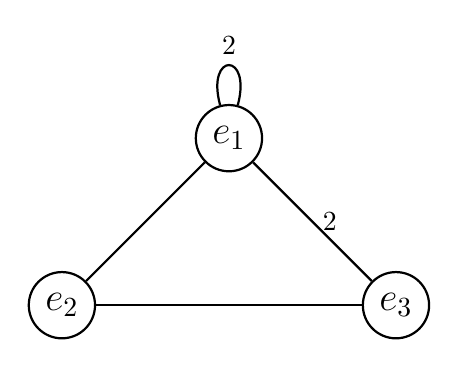
\begin{tikzpicture}[auto, node distance=3cm, every loop/.style={},
                    thick,main node/.style={circle,draw,font=\sffamily\Large\bfseries}]

  \node[main node] (1) {$e_1$};
  \node[main node] (2) [below left of=1] {$e_2$};
  \node[main node] (3) [below right of=1] {$e_3$};

  \path[every node/.style={font=\sffamily\small}];
  \path (1) edge [loop above] node {2} (1);
  \path (3) edge node [right] {} node[right] {2} (1);
  \path (1) edge (2);
  \path (2) edge (3);

\end{tikzpicture}

\caption{Graph G}

\end{center}
\end{figure}

Note - edge weights represent number of edges, default is 1.

\newpage

Question: Is G a complete bipartite graph H = (U,V,E) with the following properties:

\begin{itemize}
\item U can be a multiset
\item V can be a multiset
\item U $\cap$ V need not be empty
\end{itemize}

For the above example, the complete bipartite representation of G that we are looking for is: 
\begin{figure}[h]

\begin{center}

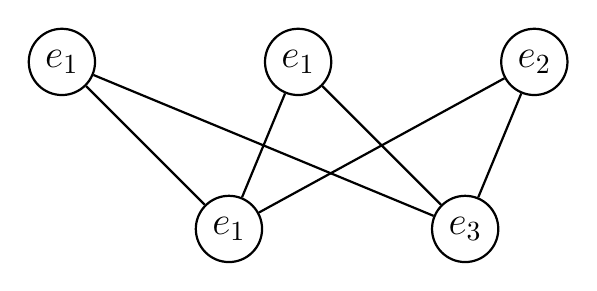
\begin{tikzpicture}[auto, node distance=3cm, every loop/.style={},
                    thick,main node/.style={circle,draw,font=\sffamily\Large\bfseries}]

  \node[main node] (1) {{$e_1$}};
  \node[main node] (2) [right of=1] {{$e_1$}};
  \node[main node] (3) [right of=2] {{$e_2$}};
  \node[main node] (4) [below right of=1] {{$e_1$}};
  \node[main node] (5) [below right of=2] {{$e_3$}};
  
  \path[every node/.style={font=\sffamily\small}];
  \path (1) edge  (4);
  \path (1) edge  (5);
  \path (2) edge  (4);
  \path (2) edge  (5);
  \path (3) edge  (4);
  \path (3) edge  (5);

\end{tikzpicture}
\caption{Graph H}

\end{center}
\end{figure}

The problem of finding whether a graph G is a complete bipartite graph under the given conditions is equivalent to finding the factors(if they exist) of a multivariate polynomial of degree 2 with no constant terms. The polynomial corresponds to the graph G whereas the factors correspond to each partition of graph H. For the above example, the multivariate polynomial is:
$(2 e_1^2 + e_1e_2 + e_2e_3 + 2 e_1e_3)$. The factors for this polynomial are $(2 e_1 + e_2)$ and $(e_1 + e_3)$.

Solving the above stated problem would give us the variables present in each operand of the long multiplication. However, we still would not know the ordering of the variables(if it exists) i.e concatenation order of the variables within the operands. We are still exploring this approach as part of our future work.


\bibliographystyle{unsrt}
\bibliography{biblio}


\end{document}

%%% Local Variables:
%%% mode: latex
%%% TeX-master: "main"
%%% End:
